% !TEX output_directory = ./build

%%%%%%%%%%%%%%%%%%%%%%%%%%%%%%%%%%%%%%%%%%%%%%%%%%%%%%%%%%%%%%%%%%%%%%%%
% Autonomous Intelligent System, University of Bonn, LaTeX Beamer theme
%
% Copyright (C) 2010-2013 Dirk Holz, dirk.holz@ieee.org

% This program is free software: you can redistribute it and/or modify
% it under the terms of the GNU General Public License as published by
% the Free Software Foundation, either version 3 of the License, or
% (at your option) any later version.

% This program is distributed in the hope that it will be useful,
% but WITHOUT ANY WARRANTY; without even the implied warranty of
% MERCHANTABILITY or FITNESS FOR A PARTICULAR PURPOSE.  See the
% GNU General Public License for more details.

% You should have received a copy of the GNU General Public License
% along with this program.  If not, see <http://www.gnu.org/licenses/>.

\documentclass[pdftex]{beamer}
\let\Tiny=\tiny

% all available options --->
% \usetheme[shadow,logoinnavbar,subsection,logoinframe,framenavbar]{AIS}
\usetheme[shadow,logoinnavbar,subsection]{AIS}

\usepackage{listings}
\usepackage{array} % needed for \arraybackslash
\usepackage{graphicx}
\usepackage{adjustbox} % for \adjincludegraphics
\usepackage{tikz}
\usetikzlibrary{shapes.geometric,shapes.arrows,decorations.pathmorphing}
\usetikzlibrary{matrix,chains,scopes,positioning,arrows,fit}
% \scalebox{<h-scale>}[<v-scale>]{<content>}


\title[Solving localization problem in first person computer games with deep learning]{Master seminar: Solving localization problem in first person computer games with deep learning}
% \subtitle{}
\author[Y.Selivonchyk]{\highlight{  Yauheni Selivonchyk}\inst{1}, \\
Prof. Dr. Christian Bauckhage\inst{2}, \\
Prof. Dr. Stefan Wrobel\inst{2}, \\
  Mr. Sc. Rafet Sifa\inst{2} \\
}
\institute[University of Bonn]
{
  \inst{1}%
  Institute of Computer Science, University of Bonn
  \and
  \inst{2}Fraunhofer IAIS
}

\date{\today}

% This is only inserted into the PDF information catalog. Can be left out.
\subject{Talks}

% Delete this, if you do not want the table of contents to pop up at
% the beginning of each subsection:
% \AtBeginSection[]
% {
%   \begin{frame}<beamer>
%     \frametitle{Outline}
%     \tableofcontents[currentsection]
%   \end{frame}
% }

% If you wish to uncover everything in a step-wise fashion, uncomment
% the following command:
% \beamerdefaultoverlayspecification{<+->}

\begin{document}

\begin{frame}
  \titlepage
\end{frame}

\begin{frame}
  \frametitle{Outline}
  \tableofcontents
  % \tableofcontents[pausesections]
\end{frame}


\section{Introduction}

\subsection{Unsupervised learning in AI}

\begin{frame}{Recent progress in AI}
  Some of the recent advances in machine learning:
  \begin{itemize}
    \item Image classification
    \item Machine translation
  \end{itemize}
  \pause
  Important attributes of it:
  \begin{itemize}
    \item Low cost and high processing abilities of modern computer chips
    \item Advances in machine learning algorithms
    \item Access to large labeled datasets
  \end{itemize}
\end{frame}

\begin{frame}{Importance of unsupervised learning for AI}
   \begin{figure}
   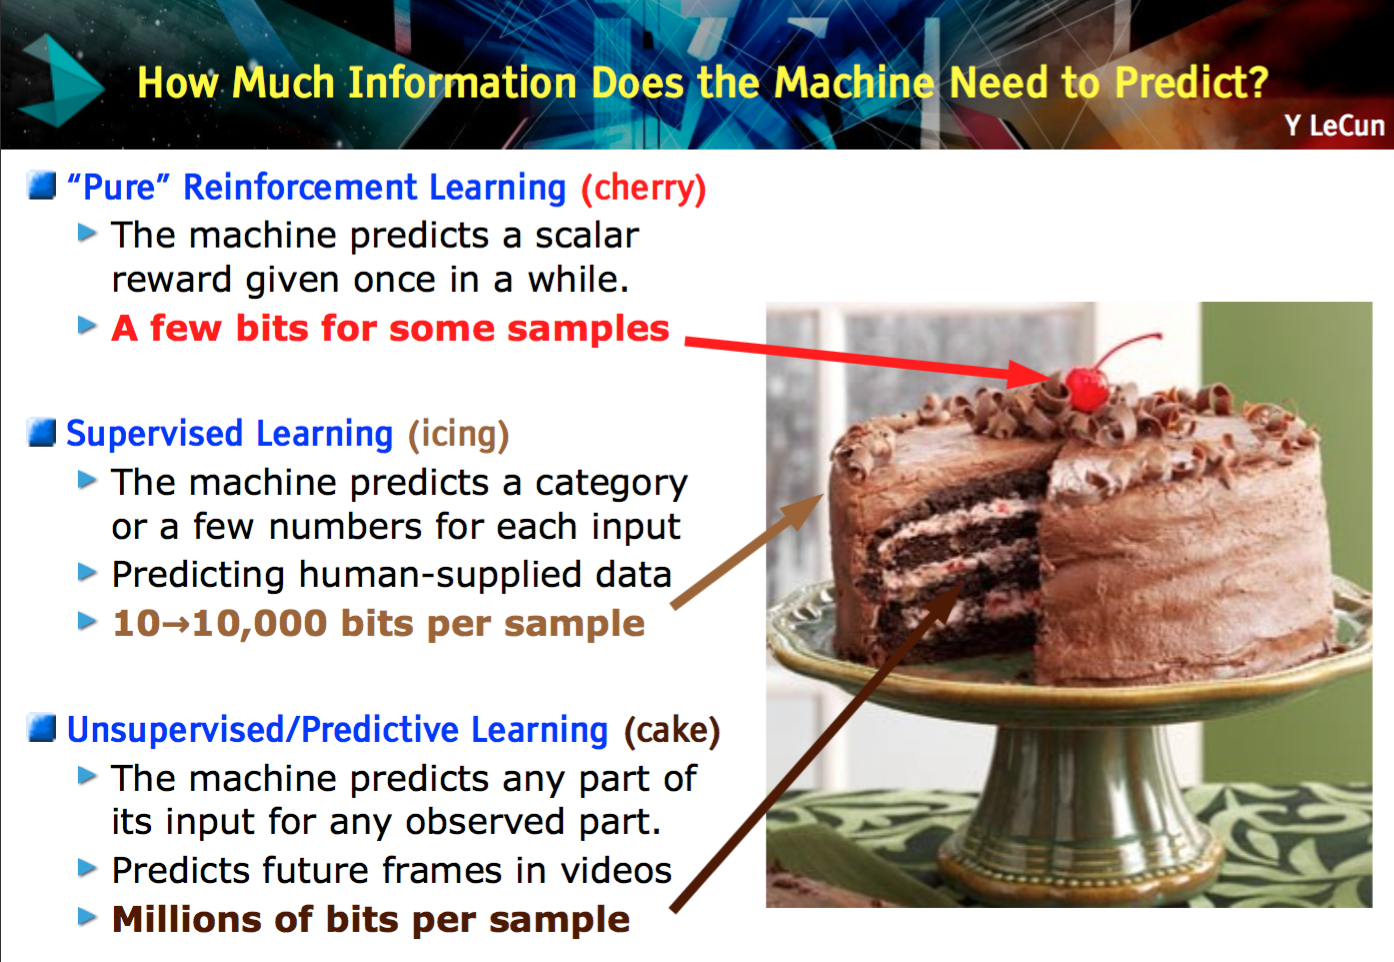
\includegraphics[width=0.8\textwidth,height=0.8\textheight,keepaspectratio]{images/lecun_nips.png}
 \caption{Slide from "Predictive learning" opening address given by Yann Lecun at NIPS2016.}
 \end{figure}
\end{frame}


\begin{frame}{Recent advances in Unsupervised learning}
  Some of the recent influential models:
  \begin{itemize}
    \item Word embedding (T. Mikolow, 2013)
    \item Variational autoencoders (D. Kingma, 2013)
    \item Generative Adversarial Networks (I. Goodfellow, 2014)
  \end{itemize}
\end{frame}


\subsection{Localization problem}


\begin{frame}{Localization}
  Localization as a task of extracting, tracking or predicting object's position in some environment from available sensory data.

  \pause
\vspace{1cm}
  Types of data:
  \begin{itemize}
    \item Visual data: images or video sequences
    \item Depth map
    \item Information about position/direction of the sensors
    \item etc.
  \end{itemize}
\end{frame}

\begin{frame}{Localization example: Tracking}
  \begin{figure}
  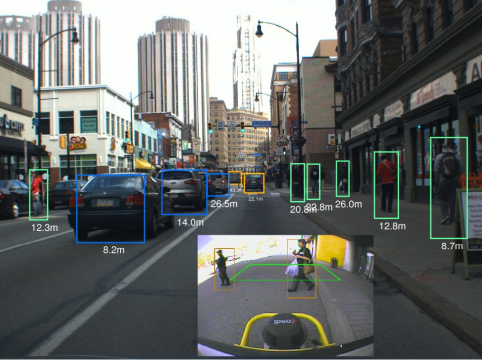
\includegraphics[width=0.5\textwidth,height=0.5\textheight,keepaspectratio]{images/tracking.png}
\caption{Pedestrian tracking visualization \footnotemark.}
\end{figure}
\footnotetext[1]{H. Cho et. al. "Real-Time Pedestrian and Vehicle Detection for Automotive Active Safety Systems"}

\end{frame}

\begin{frame}[noframenumbering]{Localization example: SLAM}
  \begin{figure}
  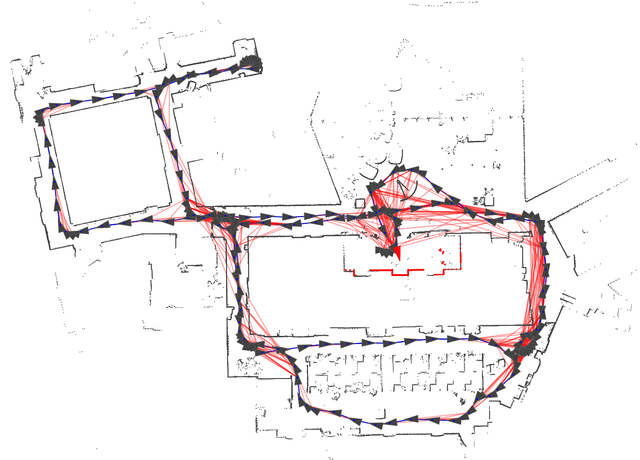
\includegraphics[width=0.8\textwidth,height=0.7\textheight,keepaspectratio]{images/slam.png}
\caption{Example solution of SLAM problem on PC3 dataset (courtesy of University of Michigan).}
\end{figure}
\end{frame}

\begin{frame}[noframenumbering]{Localization example: surgery}
  \begin{figure}
  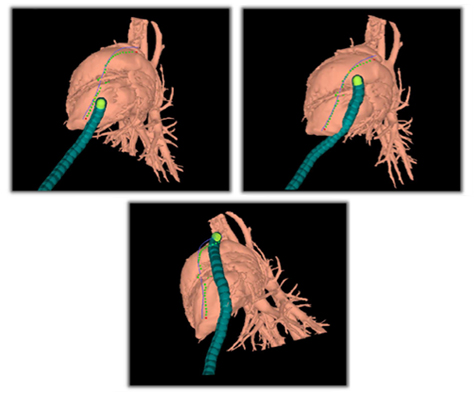
\includegraphics[width=0.8\textwidth,height=0.7\textheight,keepaspectratio]{images/slam_surg.jpg}
\caption{Mapping the position of a tool in minimally invasive surgery [http://biorobotics.ri.cmu.edu/research/medicalSLAM.html].}
\end{figure}

\end{frame}

\begin{frame}{Motivation. Continuied}
  Goal of this work: extracting interpretable low-dimensional representation of players movements in first-person shooter (games) from visual (video) data.

  \pause

  \begin{figure}
    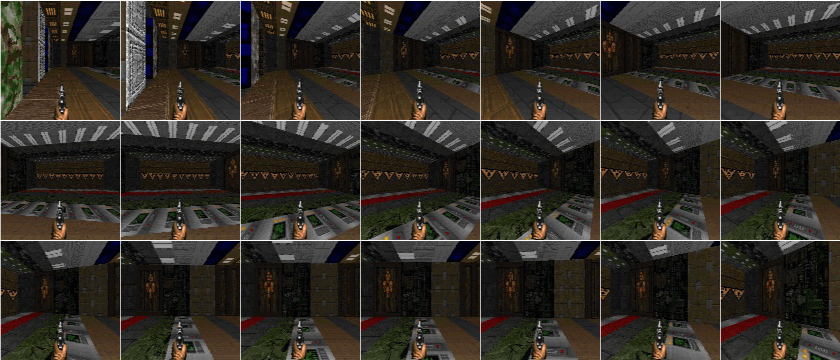
\includegraphics[width=0.8\textwidth,height=0.7\textheight,keepaspectratio]{images_main/sprite2.png}
  \caption{Example visual data.}
  \end{figure}
\end{frame}


\begin{frame}{Autoencoder model}
    \begin{tabular}{p{.5\textwidth} p{.5\textwidth}}
      $\text{Input video information:}$
      \vspace{0.5cm}
    \adjincludegraphics[width=.9\linewidth,valign=t]{images_main/sprite20.png}
    &
    $\text{Corresponding player's path:}$
    \vspace{0.5cm}
    \adjincludegraphics[width=.9\linewidth,valign=t]{images_main/cmp3/tr2.png}
    \end{tabular}
\end{frame}

% \begin{frame}{Manifold learning}
%
% \end{frame}

\begin{frame}{Example reconstructions}
    \begin{tabular}{p{.5\textwidth} p{.5\textwidth}}
      $\text{Original trajectory on the video:}$
      \vspace{0.5cm}
      \adjincludegraphics[width=.9\linewidth,valign=t]{images_main/cmp2/tr1.png}
    &
    $\text{Our embedding in a 3D space:}$
    \vspace{0.5cm}
    \adjincludegraphics[width=.9\linewidth,valign=t]{images_main/cmp2/ww_3.png}

    \end{tabular}
\end{frame}

\section{Approach}

% \subsection{Spatial embedding model}
%
% \begin{frame}
%   \begin{tabular}{p{.3\textwidth} p{.7\textwidth}}
%   \adjincludegraphics[width=.8\linewidth,valign=t]{images/slam.png}
%   &
%   \raggedright\arraybackslash\textbf{The problem of distinguishing prime numbers from composites, and of resolving composite numbers into their prime factors, is one of the most important and useful in all of arithmetic.}
%
%   \hfill-- Carl Friedrich Gauss
%   \end{tabular}
%
% \end{frame}

\subsection{Model design}

\begin{frame}{Autoencoder model}
  \textbf{Autoencoders} learn to project the input $x$ into some embedding space $h \in H$ and simultaneously reconstruct the original information $\hat{x}$.
  \pause
\vspace{1cm}

    \begin{tabular}{p{.5\textwidth} p{.5\textwidth}}
    \adjincludegraphics[width=.9\linewidth,valign=t]{images/ae2.png}
    &
    \begin{itemize}
      \item $f: \Bbb{R}^N \to \Bbb{R}^M$
      \item $g: \Bbb{R}^M \to \Bbb{R}^N$
    \end{itemize}
    \end{tabular}
\end{frame}


\begin{frame}{Autoencoder. Primary goal}
  While good quality reconstruction is desirable, we will focus on producing high quality representation in the embedding space $H$.
\vspace{1cm}

    \begin{tabular}{p{.5\textwidth} p{.5\textwidth}}
    \adjincludegraphics[width=.9\linewidth,valign=t]{images/ae2.png}
    &
    Original images and their reconstruction
    \adjincludegraphics[width=.9\linewidth,valign=t]{images/reco.png}
    \end{tabular}
\end{frame}

\begin{frame}[noframenumbering]{Autoencoder. Primary goal}
  While good quality reconstruction is desirable, we will focus on producing high quality representation in the embedding space $H$.
\vspace{1cm}

    \begin{tabular}{p{.5\textwidth} p{.5\textwidth}}
    \adjincludegraphics[width=.9\linewidth,valign=t]{images/ae2.png}
    &
    \adjincludegraphics[width=.9\linewidth,valign=t]{images/reco3.png}
    \end{tabular}
\end{frame}


\begin{frame}{Our contributions. Training process}
  \begin{itemize}
    \item We propose a robust training technique that allows unsupervised visual data embedding into extremely low dimensional space.

    Our model requires compression ratio of 10000:1, but allows information loss.
    \item We describe regularization techniques that allow to preserve spatial relations in the embedding space
  \end{itemize}
\end{frame}

\begin{frame}{Data collection}
  We use \texttt{VizDoom} scientific research platform, which is based on a 3D engine of FPS game \texttt{DoomII}.

  \begin{figure}
    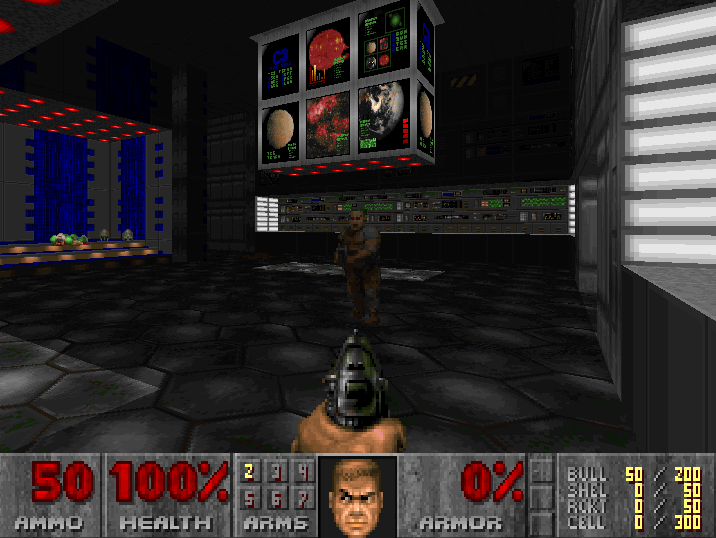
\includegraphics[width=0.62\textwidth,height=0.62\textheight,keepaspectratio]{images_main/doom.png}
    \caption{Visual data in \texttt{DoomII} computer game.}
  \end{figure}
\end{frame}


\begin{frame}{Data collection. Continued}
  We collect several trajectories for our evaluation:
  \begin{itemize}
    \item Trivial trajectories: showing simple transitions as walking along the axis with limited degress of freedom.
    \item Trajectories of natural, yet, predictable movement. As running in an \textit{eight}.
    \item Random movement on the map.
  \end{itemize}
\end{frame}

% \begin{frame}{Regularization}
% \end{frame}





\section{Evaluation}

\subsection{Metrics}

\begin{frame}{Our goals}
  Qualities of a good spatial embedding:
  \begin{itemize}
    \item It is visually interpretable;
    \item It preserves spatial structure of the trajectories in Euclidean space:
      \begin{itemize}
        \item Key trajectory elements: turns, intersections
        \item Point-to-point relations
      \end{itemize}
    \item It allows prediction of the future frames.
  \end{itemize}
\end{frame}


\begin{frame}{Prediction in the embedding space}
  Try to estimate positional encoding of the next frame using last two frames of the video.
  \begin{figure}
    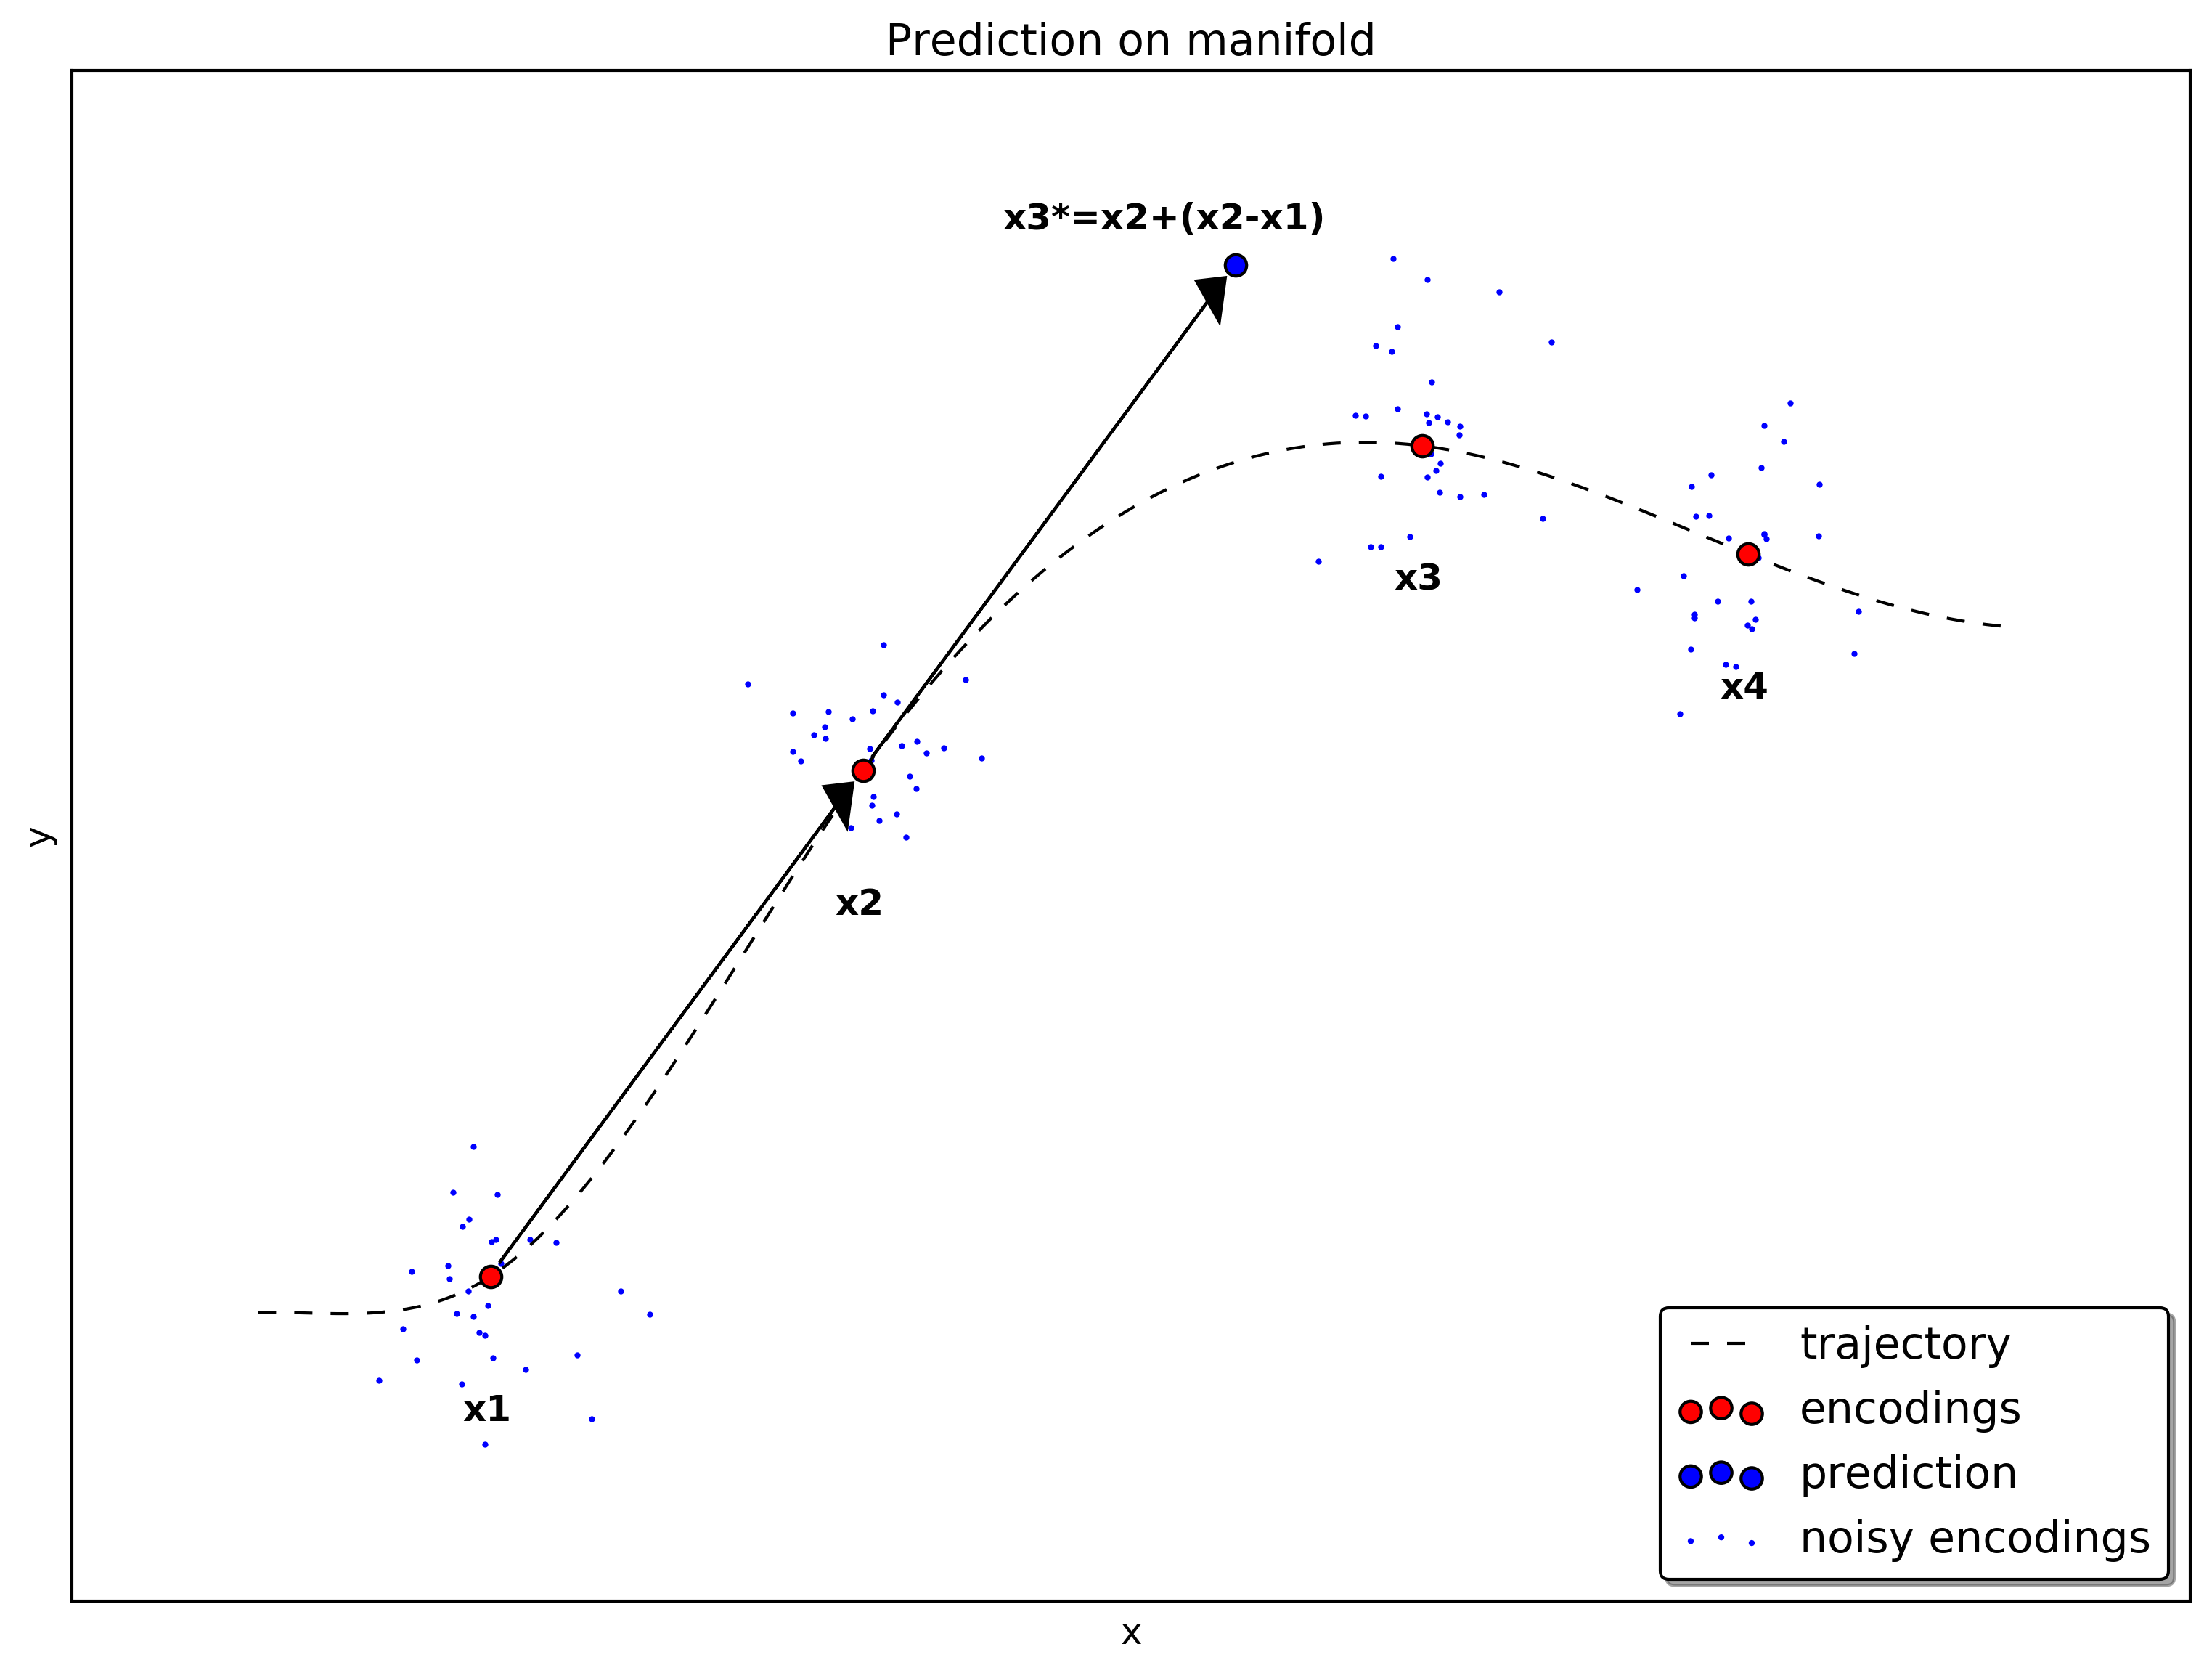
\includegraphics[width=0.75\textwidth,height=0.75\textheight,keepaspectratio]{images_main/prediction.png}
    \caption{Prediction on the spatial manifold.}
  \end{figure}
\end{frame}

\subsection{Results}

\begin{frame}{Trivial trajectory}
    \begin{tabular}{p{.5\textwidth} p{.5\textwidth}}
      $\text{Original trajectory on the video:}$
      \vspace{0.5cm}
      \adjincludegraphics[width=.9\linewidth,valign=t]{images_main/cmp2/tr1.png}
    &
    $\text{Our embedding in a 3D space:}$
    \vspace{0.5cm}
    \adjincludegraphics[width=.9\linewidth,valign=t]{images_main/fc20.png}

    \end{tabular}
\end{frame}

\begin{frame}{Trivial trajectory. Continued}
    \begin{tabular}{p{.5\textwidth} p{.5\textwidth}}
      $\text{Trajectory:}$
      \vspace{0.5cm}
      \adjincludegraphics[width=.9\linewidth,valign=t]{images_main/fc20.png}
    &
    Key characteristics
    \begin{itemize}
      \item Trajectory is visually recognizable
      \item Subsequent frames remain nearest neighbors 78\% of the time
      \item Predicted frames are on average 37\% closer to actual embedding comparing to current frame
    \end{itemize}
    \end{tabular}
\end{frame}


\begin{frame}{Natural trajectory}
    \begin{tabular}{p{.5\textwidth} p{.5\textwidth}}
      $\text{Original trajectory on the video:}$
      \vspace{0.5cm}
      \adjincludegraphics[width=.9\linewidth,valign=t]{images_main/cmp3/tr2.png}
    &
    $\text{Our embedding in a 3D space:}$
    \vspace{0.5cm}
    \adjincludegraphics[width=.9\linewidth,valign=t]{images_main/cmp3/cnn4_2.png}

    \end{tabular}
\end{frame}

\begin{frame}{Natural trajectory. Continued}
    \begin{tabular}{p{.5\textwidth} p{.5\textwidth}}
      $\text{Trajectory embedding:}$
      \vspace{0.5cm}
      \adjincludegraphics[width=.9\linewidth,valign=t]{images_main/cmp3/cnn4_2.png}
    &
    Key characteristics
    \begin{itemize}
      \item Trajectory is hard to recognize
      \item Subsequent frames remain nearest neighbors 91\% of the time
      \item Predicted frames are on average 58\% closer to actual embedding comparing to the current frame
    \end{itemize}
    \end{tabular}
\end{frame}

% \begin{frame}{General trajectory}
%     \begin{tabular}{p{.5\textwidth} p{.5\textwidth}}
%       $\text{Original trajectory on the video:}$
%       \vspace{0.5cm}
%       \adjincludegraphics[width=.9\linewidth,valign=t]{images_main/cmp3/tr2.png}
%     &
%     $\text{Our embedding in a 3D space:}$
%     \vspace{0.5cm}
%     \adjincludegraphics[width=.9\linewidth,valign=t]{images_main/cmp4/cnn8_3.png}
%
%     \end{tabular}
% \end{frame}


\begin{frame}[noframenumbering]{General trajectory}
    \begin{tabular}{p{.5\textwidth} p{.5\textwidth}}
      $\text{Original trajectory on the video:}$
      \vspace{0.5cm}
      \adjincludegraphics[width=.9\linewidth,valign=t]{images_main/cmp3/tr2.png}
    &
    $\text{Our embedding in a 3D space:}$
    \vspace{0.5cm}
    \adjincludegraphics[width=.9\linewidth,valign=t]{images_main/cmp4/cnn8_3.png}

    \end{tabular}
\end{frame}

\begin{frame}[noframenumbering]{General trajectory}
    \begin{tabular}{p{.5\textwidth} p{.5\textwidth}}
      $\text{Original trajectory on the video:}$
      \vspace{0.5cm}
      \adjincludegraphics[width=.9\linewidth,valign=t]{images_main/cmp2/tr1.png}
    &
    $\text{Our embedding in a 3D space:}$
    \vspace{0.5cm}
    \adjincludegraphics[width=.9\linewidth,valign=t]{images_main/cmp4/cnn8.png}

    \end{tabular}
\end{frame}

\begin{frame}{General trajectory. Continued}
    \begin{tabular}{p{.5\textwidth} p{.5\textwidth}}
      $\text{Trajectory embedding:}$
      \vspace{0.5cm}
      \adjincludegraphics[width=.9\linewidth,valign=t]{images_main/cmp4/cnn8_3.png}
    &
    Key characteristics
    \begin{itemize}
      \item Trajectory is not recognizable
      \item Subsequent frames remain nearest neighbors 58\% of the time
      \item Only 19\% of predicted frames were at least somewhat closer to the actual embedding than current frame
    \end{itemize}
    \end{tabular}
\end{frame}


\section*{Summary}

\begin{frame}
  \frametitle<presentation>{Summary}

  \begin{itemize}
  \item We proposed a model for unsupervised learning of topological trajectory from first-person video
  \item We successfully trained the model on trajectories of various complexities
  \item We identified the limits of our model depending on the complexity of training concepts
  \end{itemize}

%   % The following outlook is optional.
  \vskip0pt plus.5fill
  \begin{itemize}
  \item Shortcomings:
    \begin{itemize}
    \item The embedding is not robust against some common transformations.
    \item Current concept do not allow to separate positional information of the player from direction of players view.
    \end{itemize}
  \end{itemize}
\end{frame}

\begin{frame}{Future work}

  \begin{itemize}
  \item Manifold
  \end{itemize}

  % The following outlook is optional.
  \vskip0pt plus.5fill
  \begin{itemize}
  \item Outlook
    \begin{itemize}
    \item Something you haven't solved.
    \item Something else you haven't solved.
    \end{itemize}
  \end{itemize}
\end{frame}

\end{document}
